\section{Necesidades del negocio}

\begin{textoazul}
Esta sección obligatoria debe contener información sobre los objetivos de negocio de clientes y usuarios, incluyendo los modelos de procesos de negocio a implantar. Esta sección se divide en las secciones que se describen a continuación.

La información de esta sección puede que ya se encuentre total o parcialmente en documentación previa como el Pliego de Prescripciones Técnicas, la Oferta seleccionada o el Estudio de Viabilidad del Sistema, en cuyo se podrá reutilizar y se hará referencia a dichos documentos como fuente de la misma.
\end{textoazul}
 
\subsection{Objetivos de Negocio}
\begin{textoazul}
Esta sección debe contener los objetivos de negocio que se esperan alcanzar cuando el sistema software a desarrollar esté en producción, especificados mediante las  plantillas de objetivos de negocio que se muestran a continuación. En el caso de que se considere necesario, los objetivos de negocio se pueden descomponer jerárquicamente para facilitar su comprensión y representar dicha jerarquía de forma gráfica.
 \end{textoazul}




 \begin{Artefacto}[H]
    \centering
    \begin{tabular}{|p{3cm}|p{10cm}|}
        \hline
         \cellcolor{gray30}  NEG-OBJ 999	&  $<$nombre descriptivo$>$\\ 
%      \cellcolor{gray30}  BUS-OBJ 999	& <descriptive name>\\   
        \hline
         \cellcolor{gray30}  [Versión]	&  $<$nº versión$>$($<$fecha de versión$>$)\\   
%      \cellcolor{gray30}  [Version]	&   $<$nº version$>$($<$date$>$)\\   
         \hline
         \cellcolor{gray30}  [Dependencias] &  	\begin{itemize} \item $<procesos de negocio actuales en los que participa>$
\item	... \end{itemize}\\  
%                 \cellcolor{gray30}  [Dependencies] &  	\begin{itemize} \item $<business processes this actor is involved in>$
%\item	... \end{itemize}\\            
        \hline
        \cellcolor{gray30} Descripción	& Este objetivo representa  \\
%      \cellcolor{gray30}   Description	& descrip\\   
        \hline
                 \cellcolor{gray30}  Subobjetivos &  	\begin{itemize} \item $<objetivos del negocio hijos>$
\item	... \end{itemize}\\  
%                 \cellcolor{gray30}  [Subobjectives] &  	\begin{itemize} \item<subobjetives >$
%\item	... \end{itemize}\\            
        \hline
         \cellcolor{gray30}Importancia	& $<importancia del proceso de negocio para el cliente>$  \\
%      \cellcolor{gray30}   Importance 	& descrip\\   
        \hline
          \cellcolor{gray30}  [Prioridad] &  	$<prioridad del objetivo de negocio para la direccion$ $ del proyecto>$\\
%                 \cellcolor{gray30}  [Priority] &   	\\
         \hline
         \cellcolor{gray30}  Comentarios	&$<comentarios adicionales sobre el actor de negocio actual>$\\   
%         \cellcolor{gray30} Comments	&$<additional comments>$
        \hline
  
    \end{tabular}
\caption{NEG-OBJ 999	$<nombre descriptivo>$ }
%\caption{BUS-OBJ 999	$<descriptive name>$ }
  \end{Artefacto}


\subsection{Modelos de Procesos de Negocio a Implantar} 

\begin{textoazul}
Esta sección opcional, debe contener los modelos de procesos de negocio a implantar, que normalmente son los modelos de procesos de negocio actuales con ciertas mejoras. Si las diferencias con los modelos de procesos actuales son pequeñas, se puede optar por describir únicamente dichas diferencias siempre que se hayan incluido los modelos de procesos actuales en la sección 3.2.
\end{textoazul}
 
 
 
 \begin{Artefacto}[H]
 \centering
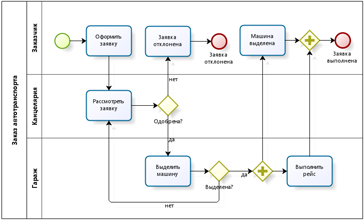
\includegraphics[width=0.8\textwidth]{\fig/BPMN.png}
 \caption{NEG-MOD 999	$<nombre descriptivo>$}
 \end{Artefacto}
 
\subsubsection{Descripción de los Actores de Negocio a Implantar}

 
 \begin{Artefacto}[H]
    \centering
    \begin{tabular}{|p{3cm}|p{10cm}|}
        \hline
         \cellcolor{gray30}  NEG-ACT 999	&  $<nombre descriptivo>$\\ 
%      \cellcolor{gray30}  BUS-ACt 999	& <descriptive name>\\   
        \hline
         \cellcolor{gray30}  [Versión]	&  $<$nº versión$>$($<$fecha de versión$>$)\\   
%      \cellcolor{gray30}  [Version]	&   $<$nº version$>$($<$date$>$)\\   
         \hline
         \cellcolor{gray30}  [Dependencias] &  	\begin{itemize} \item $<procesos de negocio  en los que participara>$
\item	... \end{itemize}\\  
%                 \cellcolor{gray30}  [Dependencies] &  	\begin{itemize} \item $<business processes this actor will be involved in>$
%\item	... \end{itemize}\\            
        \hline
         \cellcolor{gray30} Descripción	& Este actor de negocio  representa a $<descripcion de la organizacion, rol  o responsabilidad$ $  a la que representa  el actor de negocio a implantar>$  \\
%      \cellcolor{gray30}   Description	& descrip\\   
        \hline
         \cellcolor{gray30}  Comentarios	&$<comentarios adicionales actor de negocio  a implantar>$\\   
%         \cellcolor{gray30} Comments	&$<additional comments>$
        \hline
  
    \end{tabular}
\caption{NEG-ACT 999	$<nombre descriptivo>$ }
%\caption{BUS-ACT 999	$<descriptive name>$ }
  \end{Artefacto}




\subsubsection{Descripción de Procesos de Negocio a Implantar}
 

 \begin{Artefacto}[H]
    \centering
    \begin{tabular}{|p{3cm}|p{10cm}|}
        \hline
         \cellcolor{gray30}  NEG-PRO 999	&  $<nombre descriptivo>$\\ 
%      \cellcolor{gray30}  BUS-PRO 999	& <descriptive name>\\   
        \hline
         \cellcolor{gray30}  [Versión]	&  $<$nº versión$>$($<$fecha de versión$>$)\\   
%      \cellcolor{gray30}  [Version]	&   $<$nº version$>$($<$date$>$)\\   
         \hline
         \cellcolor{gray30}  [Dependencias] &  	\begin{itemize} \item $<procesos de negocio a implantar $ $en los que participa>$
\item	... \end{itemize}\\  
%                 \cellcolor{gray30}  [Dependencies] &  	\begin{itemize} \item $<$business processes this actor is involved in$>$
%\item	... \end{itemize}\\            
        \hline
        \cellcolor{gray30} Descripción	& Este procesos  \\
%      \cellcolor{gray30}   Description	& descrip\\   
        \hline
         \cellcolor{gray30}[Importancia]	& $<importancia del proceso de negocio para el cliente>$  \\
%      \cellcolor{gray30}   Importance 	& descrip\\   
        \hline
           \cellcolor{gray30}  [Actores] &  	\begin{itemize} \item $<actor que participa en el proceso $ $de negocio implantar>$
\item	... \end{itemize}\\  
%                 \cellcolor{gray30}  [Actors] &  	\begin{itemize} \item $<$actor involved in the business process$>$
%\item	... \end{itemize}\\
         \hline
         \cellcolor{gray30}  Comentarios	&$<comentarios adicionales del actor$ $ de negocio a implantar>$\\   
%         \cellcolor{gray30} Comments	&$<$additional comments$>$
        \hline
  
    \end{tabular}
\caption{NEG-PRO 999	$<$nombre descriptivo$>$ }
%\caption{BUS-PRO 999	$<$descriptive name $>$ }
  \end{Artefacto}
